% Concrete instance of the square-root image separation used in Chapter 10.
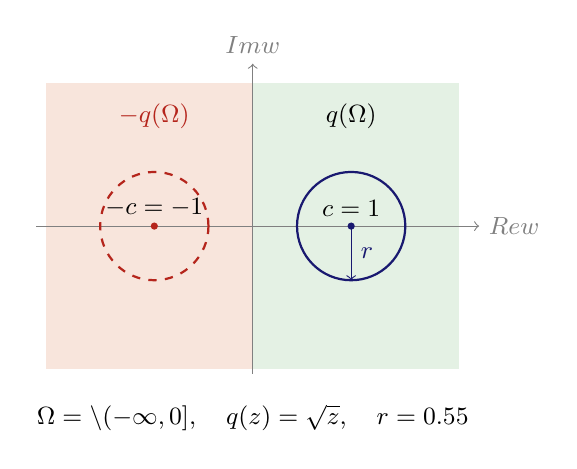
\begin{tikzpicture}[x=1.25cm,y=1.25cm,font=\small]
\fill[ForestGreen!12] (0,-1.45) rectangle (2.1,1.45);
\fill[BrickRed!9] (-2.1,-1.45) rectangle (0,1.45);
\draw[->,gray] (-2.2,0)--(2.3,0) node[right] {$\operatorname{Re}w$};
\draw[->,gray] (0,-1.5)--(0,1.65) node[above] {$\operatorname{Im}w$};
\draw[MidnightBlue,thick] (1,0) circle (.55);
\draw[BrickRed,thick,dashed] (-1,0) circle (.55);
\fill[MidnightBlue] (1,0) circle (1.3pt);
\fill[BrickRed] (-1,0) circle (1.3pt);
\node[above] at (1,0) {$c=1$};
\node[above] at (-1,0) {$-c=-1$};
\draw[MidnightBlue,->] (1,0)--(1,-.55) node[midway,right] {$r$};
\node[align=center] at (1,1.12) {$q(\Omega)$};
\node[BrickRed,align=center] at (-1,1.12) {$-q(\Omega)$};
\node[align=center] at (0,-1.95) {$\Omega=\C\setminus(-\infty,0],\quad q(z)=\sqrt z,\quad r=0.55$};
\end{tikzpicture}
